\begin{frame}{Das Vertrauensproblem in der Praxis}
	Eine mathematisch korrekte RSA-Signatur beweist \textbf{Integrität} und den Besitz des privaten Schlüssels.
	
	\begin{alertblock}{Die fundamentale Vertrauensfrage}
		\emph{Woher weiss der Empfänger (Bob), dass ein bestimmter öffentlicher Schlüssel tatsächlich Alice (oder der Bank) gehört?}
	\end{alertblock}
	
	\begin{itemize}[<+->]
		\item \textbf{Man-in-the-Middle-Angriff}:
		      Eve generiert ein eigenes Schlüsselpaar $(e_E, d_E)$ und gibt vor, Alice zu sein.
		\item Signiert Eve eine gefälschte Nachricht mit $d_E$, so bestätigt Bobs Prüfung mit $e_E$ formal die Gültigkeit der Signatur.
		\item \textbf{Ergebnis}: Bob wiegt sich in falscher Sicherheit, da er den Schlüssel nicht der realen Identität zuordnen kann!
	\end{itemize}
\end{frame}

\begin{frame}{Lösung: Digitale Zertifikate \& PKI}
	Um die Identität von Schlüsselinhabern zweifelsfrei zu bestätigen, nutzen wir eine \textbf{Public-Key-Infrastruktur} (\acrshort{PKI}):
	
	\begin{mydefinition}[Komponenten einer PKI]
		{\small
		\begin{itemize}[<+->]
			\item \textbf{Zertifizierungsstelle (\emph{Certificate Authority}, \acrshort{CA})}:
			      Eine vertrauenswürdige Institution, die vor der Schlüsselausgabe die reale Identität prüft.
			\item \textbf{Digitales Zertifikat}:
			      Ein elektronisches Dokument, das die Identität an den öffentlichen Schlüssel bindet und von der \acrshort{CA} digital signiert ist:
			      \[ \text{Cert}_A := z^{d_{\text{CA}}} \bmod n_{\text{CA}} \qquad \text{mit } z = (\text{\enquote{Alice}}, e_A, n_A) \]
			\item \textbf{Vertrauensanker (Root-\acrshort{CA})}:
			      Betriebssysteme und Browser besitzen einen vorinstallierten Speicher vertrauenswürdiger Stammzertifikate (\emph{Trust Store}).
		\end{itemize}
		}
	\end{mydefinition}
\end{frame}

\begin{frame}{Zweistufige Verifikation mit PKI}
	\begin{figure}[H]
		\centering
		\resizebox{!}{0.75\textheight}{\begin{tikzpicture}[
	scale=0.78, every node/.style={transform shape},
	actor/.style={rectangle, rounded corners, draw=black, fill=gray!15, minimum width=3.4cm, minimum height=1.1cm, font=\bfseries, align=center, inner sep=4pt},
	stepbox/.style={rectangle, rounded corners, draw=#1, fill=#1!8, line width=0.8pt, font=\small, align=center, inner sep=6pt},
	msgarrow/.style={->, >=stealth, line width=1pt, #1},
	badge/.style={circle, fill=#1, text=white, font=\bfseries\footnotesize, inner sep=2pt}
]
	% Spaltenkoordinaten
	\def\colA{0}     % Alice
	\def\colCA{5.5}  % CA
	\def\colB{11}    % Bob

	% --- AKTEURE (Kopfzeile) ---
	\node[actor] (alice) at (\colA, 0) {Alice\\{\footnotesize (Absenderin)}\\[2pt]{\scriptsize öff.: $(e_A, n_A)$,\; priv.: $d_A$}};
	\node[actor, fill=DarkOrchid!15, draw=DarkOrchid] (ca) at (\colCA, 0) {\textcolor{DarkOrchid}{\faCertificate{}} CA\\{\footnotesize (Zertifizierungsstelle)}\\[2pt]{\scriptsize öff.: $(e_{\text{CA}}, n_{\text{CA}})$,\; priv.: $d_{\text{CA}}$}};
	\node[actor] (bob) at (\colB, 0) {Bob\\{\footnotesize (Empfänger)}\\[2pt]{\scriptsize vorinstalliert: $(e_{\text{CA}}, n_{\text{CA}})$}};

	% Vertikale Hilfslinien
	\draw[dashed, gray!40] (alice.south) -- (\colA, -13.8);
	\draw[dashed, gray!40] (ca.south) -- (\colCA, -5.8);
	\draw[dashed, gray!40] (bob.south) -- (\colB, -13.8);

	% --- PHASE 1: ZERTIFIZIERUNG (VORAB) ---
	\node[font=\footnotesize\bfseries\color{DarkOrchid!80!black}, fill=white, inner sep=2pt] at (\colCA, -1.1) {Phase 1: Zertifikatserstellung (einmalig vorab)};

	% Pfeil 1: Alice -> CA (Schlüsselregistrierung)
	\node[badge=RoyalBlue] (b1) at (\colA+0.6, -2.0) {1};
	\draw[msgarrow=RoyalBlue] (b1.east) -- (\colCA-0.3, -2.0)
		node[midway, above=2pt, font=\footnotesize] {Antrag mit Daten $z = (\text{\enquote{Alice}}, e_A, n_A)$};

	% CA signiert
	\node[stepbox=DarkOrchid] (ca_sign) at (\colCA, -3.4) {
		\textbf{CA prüft Identität \& signiert $z$:}\\
		$\text{Cert}_A := z^{d_{\text{CA}}} \bmod n_{\text{CA}}$
	};

	% Pfeil 2: CA -> Alice (Zertifikatsausgabe)
	\node[badge=DarkOrchid] (b2) at (\colCA-0.6, -4.8) {2};
	\draw[msgarrow=DarkOrchid] (b2.west) -- (\colA+0.3, -4.8)
		node[midway, above=2pt, font=\footnotesize] {Ausgabe: Zertifikat $(z, \text{Cert}_A)$};

	% --- PHASE 2: VERSAND DER SIGNIERTEN NACHRICHT ---
	\node[font=\footnotesize\bfseries\color{RoyalBlue!80!black}, fill=white, inner sep=2pt] at (5.5, -6.0) {Phase 2: Signieren \& Übertragen};

	% Alice signiert
	\node[stepbox=RoyalBlue] (alice_sign) at (\colA, -7.3) {
		\textbf{Alice signiert Vertrag $m$:}\\
		$s := m^{d_A} \bmod n_A$
	};

	% Pfeil 3: Alice -> Bob
	\node[badge=black] (b3) at (\colA+1.8, -9.0) {3};
	\draw[msgarrow=black] (b3.east) -- (\colB-1.8, -9.0)
		node[midway, above=3pt, font=\footnotesize, align=center] {Vertrag $m$ \quad+\quad Signatur $s$ \quad+\quad Zertifikat $(z, \text{Cert}_A)$};

	% --- PHASE 3: ZWEISTUFIGE VERIFIKATION BEI BOB ---
	\node[font=\footnotesize\bfseries\color{ForestGreen!80!black}, fill=white, inner sep=2pt] at (\colB, -10.3) {Phase 3: Verifikation bei Bob};

	% Bob Verifikation
	\node[stepbox=ForestGreen] (bob_verify) at (\colB, -12.1) {
		\textbf{Schritt A: Zertifikat mit $(e_{\text{CA}}, n_{\text{CA}})$ prüfen}\\
		$z' := (\text{Cert}_A)^{e_{\text{CA}}} \bmod n_{\text{CA}}$\\
		$\rightarrow \text{Gilt } z' = z\text{?} \implies (e_A, n_A)\text{ ist echt!}$\\[4pt]
		\textbf{Schritt B: Signatur mit $(e_A, n_A)$ prüfen}\\
		$m' := s^{e_A} \bmod n_A$\\
		$\rightarrow \text{Gilt } m' = m\text{?} \implies \text{Vertrag ist echt!} \textcolor{ForestGreen}{\mathbf{\checkmark}}$
	};
\end{tikzpicture}
}
	\end{figure}
\end{frame}

\begin{frame}{Auftrag: Zertifizierte digitale Signaturen}
	 \aufgabebox{Lösen Sie Aufgabe 5.1 im Skript (Zertifikat)}
\end{frame}

\begin{frame}{Die Vertrauenskaskade: Zertifikatskette}
	In der Praxis signiert eine Root-\acrshort{CA} fast nie direkt einzelne Server-Zertifikate, sondern nutzt Zwischenzertifikate:
	
	\begin{figure}[H]
		\centering
		\resizebox{0.82\linewidth}{!}{\begin{tikzpicture}[
	scale=0.82, every node/.style={transform shape},
	box/.style={rectangle, rounded corners=4pt, draw=#1, fill=#1!10, line width=1pt, align=center, inner sep=5pt, font=\small},
	chainarrow/.style={->, >=stealth, line width=1.1pt, #1}
]
	% Hierarchie-Knoten
	\node[box=DarkOrchid, minimum width=9.5cm] (root) at (0, 3.6) {
		\textbf{\textcolor{DarkOrchid}{\faKey{} Root-CA: \texttt{Amazon Root CA 1} / \texttt{SwissSign Gold CA - G2}}}\\
		{\scriptsize \faShield*{} Vorinstalliert im Trust Store $\cdot$ Privater Schlüssel offline (Air-Gapped)}
	};

	\node[box=RoyalBlue, minimum width=9.5cm] (inter) at (0, 1.8) {
		\textbf{\textcolor{RoyalBlue}{\faCertificate{} Intermediate-CA: \texttt{Amazon RSA 2048 M04} / \texttt{Swiss Government PKI}}}\\
		{\scriptsize Signiert von der Root-CA $\cdot$ Operative Zertifikatsausgabe}
	};

	\node[box=ForestGreen, minimum width=9.5cm] (leaf) at (0, 0.0) {
		\textbf{\textcolor{ForestGreen}{\faServer{} Server-Zertifikat: \texttt{www.sbb.ch} / \texttt{www.admin.ch}}}\\
		{\scriptsize Signiert von der Intermediate-CA $\cdot$ Öffentlicher Schlüssel der Website}
	};

	\node[box=gray, minimum width=9.5cm, fill=gray!8] (client) at (0, -1.8) {
		\textbf{\faLaptop{} Webbrowser / Betriebssystem (Client)}\\
		{\scriptsize Prüft Signaturkette von unten nach oben bis zum vorinstallierten Root-Zertifikat}
	};

	% Pfeile (Signaturfluss von oben nach unten)
	\draw[chainarrow=DarkOrchid] (root.south) -- (inter.north)
		node[midway, right=6pt, font=\footnotesize] {signiert Zwischenzertifikat};
	\draw[chainarrow=RoyalBlue] (inter.south) -- (leaf.north)
		node[midway, right=6pt, font=\footnotesize] {signiert Server-Zertifikat};
	\draw[chainarrow=ForestGreen] (leaf.south) -- (client.north)
		node[midway, right=6pt, font=\footnotesize] {überträgt Zertifikatkette bei \gls{HTTPS}};

	% Prüfpfeil rückwärts links
	\draw[->, >=stealth, dashed, line width=1.1pt, BrickRed] (client.west) to[out=168, in=192] node[midway, left=4pt, font=\scriptsize\bfseries, align=center, rotate=90] {Kryptographische Verifikation} (root.west);

\end{tikzpicture}
}
	\end{figure}
	
	\begin{itemize}
		\item \textbf{Sicherheitsvorteil}: Der private Root-Schlüssel bleibt streng isoliert \emph{offline} (Air-Gapped). Bei einem Zwischenfall muss nur das Intermediate-Zertifikat widerrufen werden.
	\end{itemize}
\end{frame}

\begin{frame}{Zertifikatsinspektion im Webbrowser (SBB)}
	\begin{columns}[T]
		\begin{column}{0.55\textwidth}
			\centering
			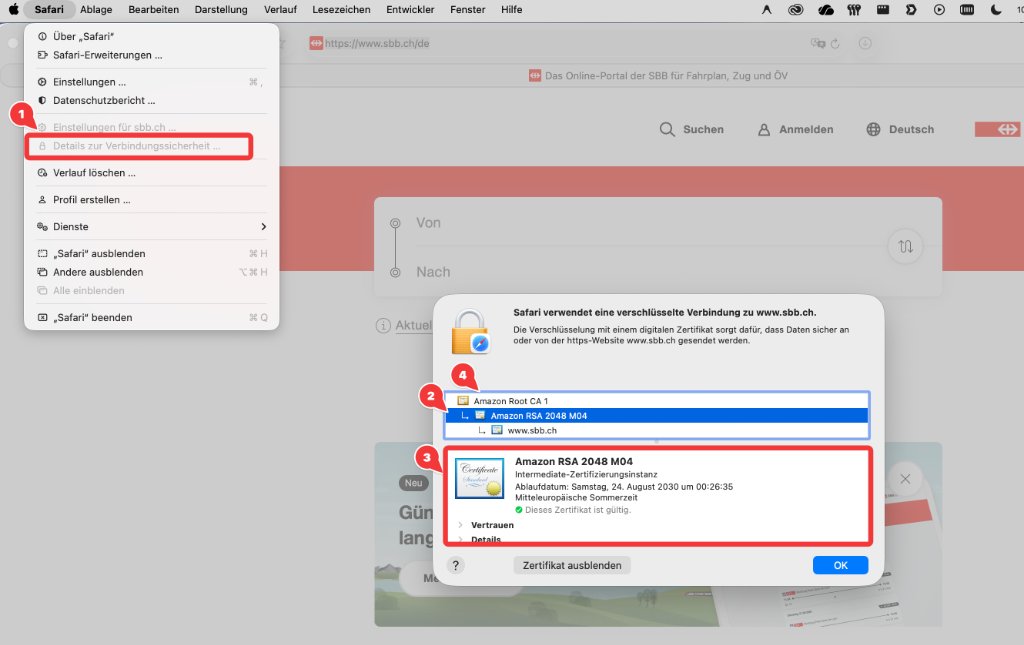
\includegraphics[width=\linewidth]{Grundlagen_Info/03_Kryptologie/Figures/certificate_hierarchy_sbb}
		\end{column}
		\begin{column}{0.45\textwidth}
			{\small
			\textbf{Zertifikatsaufbau bei \url{https://www.sbb.ch}:}
			\begin{enumerate}
				\item \textbf{Root-\acrshort{CA}}: \texttt{Amazon Root CA 1} (im Betriebssystem vorinstalliert).
				\item \textbf{Intermediate-\acrshort{CA}}: \texttt{Amazon RSA 2048 M04}.
				\item \textbf{Blatt-Zertifikat}: \texttt{www.sbb.ch} (Inhaberin: Schweizerische Bundesbahnen).
			\end{enumerate}
			\medskip
			\textbf{Verschlüsselung}: TLS mit AES / RSA / ECC.
			}
		\end{column}
	\end{columns}
\end{frame}

\begin{frame}{Elektronische Signaturen in der Schweiz (ZertES)}
	\begin{block}{Bundesgesetz über die elektronische Signatur (\acrshort{ZertES})}
		{\small
		In der Schweiz regelt das \textbf{ZertES} die rechtliche Gültigkeit von elektronischen Signaturen:
		\begin{itemize}[<+->]
			\item \textbf{Qualifizierte elektronische Signatur (QES)}:
			      Ist der eigenhändigen handschriftlichen Unterschrift rechtlich vollständig gleichgestellt (Art.~14 Abs.~$2^{\text{bis}}$ OR).
			\item \textbf{Anerkannte Vertrauensdienste in der Schweiz}:
			      \begin{itemize}
				      \item \textbf{SwissSign}: Schweizerische Post / SwissID (z.\,B.\ für Verträge und eGovernment).
				      \item \textbf{Swisscom Trust Services}: Signaturdienste für Banken und Unternehmen.
				      \item \textbf{SWITCHpki}: Zertifikate für Schweizer Universitäten und Schulen.
				      \item \textbf{Swiss Government PKI}: Interne PKI für die Bundesverwaltung.
			      \end{itemize}
		\end{itemize}
		}
	\end{block}
\end{frame}

\begin{frame}{Auftrag: Zertifikats-Detektiv im Browser}
	\begin{itemize}
		\item \aufgabebox{Aufgabe 5.2 im Skript (Zertifikats-Detekti)}
		\item \textbf{Challenge}: Öffnen Sie Safari, Chrome, Edge oder Firefox und inspizieren Sie die Zertifikate von \url{https://www.sbb.ch}, \url{https://www.admin.ch} oder Ihrer Schule.
	\end{itemize}
\end{frame}
